\documentclass[slide,papersize]{jsarticle}
\usepackage[dvipdfmx]{graphicx,color}
\begin{document}

\section*{センサ等}
\vspace*{13mm}
\begin{center}
{\Huge {\bf 特殊な\\入力デバイス}}
\end{center}

\section*{agenda}
\bigskip
\begin{itemize}
\item 音声入力
\bigskip
\item GPS
\bigskip
\item カメラ
\bigskip
\item 各種センサ
\end{itemize}

\section*{音声入力}
\bigskip
\begin{itemize}
\item google な Android デバイス (?) のみ
\bigskip
\item 音声検索 api の導入必須
\end{itemize}

\section*{サンプル確認}
\bigskip
\begin{itemize}
\item http://db.tt/ETXCOa
\bigskip
 \begin{itemize}
 \item ファイル取得
 \item Eclipse に import
 \item 内容確認してみましょう
 \end{itemize}
\bigskip
 \begin{itemize}
 \item Intent に渡している定数
 \item ACTION\_RECOGNIZE\_SPEECH
 \item ACTION\_WEB\_SEARCH
 \end{itemize}
\end{itemize}

\section*{実機で動作確認}
\bigskip
\begin{itemize}
\item 実機でないと動作確認できません
\end{itemize}

\section*{GPS}
\bigskip
\begin{itemize}
\item permission の設定
\bigskip
\item データ取得手順
\end{itemize}

\section*{permission}
\bigskip
\begin{itemize}
\item \begin{verbatim}ACCESS_FINE_LOCATION の追加\end{verbatim}
\bigskip
\item エミュレータで試験する場合
 \begin{itemize}
 \item \begin{verbatim}ACCESS_MOCK_LOCATION の追加\end{verbatim}
 \end{itemize}
\end{itemize}

\section*{実装}
\bigskip
\begin{itemize}
\item Activity に LocationListener 実装
\bigskip
\item メソッド実装
 \begin{itemize}
 \item {\scriptsize GPS イベントのコールバック}
 \item {\scriptsize \begin{verbatim}主に LocationListener#onLocationChanged()\end{verbatim}}
 \end{itemize}
\bigskip
\item {\scriptsize \begin{verbatim}Activity#getSystemService() で LocationManager 取得\end{verbatim}}
\bigskip
\item {\scriptsize \begin{verbatim}LocationManager#requestLocationUpdates() 呼び出し\end{verbatim}}
\end{itemize}

\section*{実装例}
{\footnotesize こんなカンジ? (これだけだと未だ何もしません)}
\begin{center}
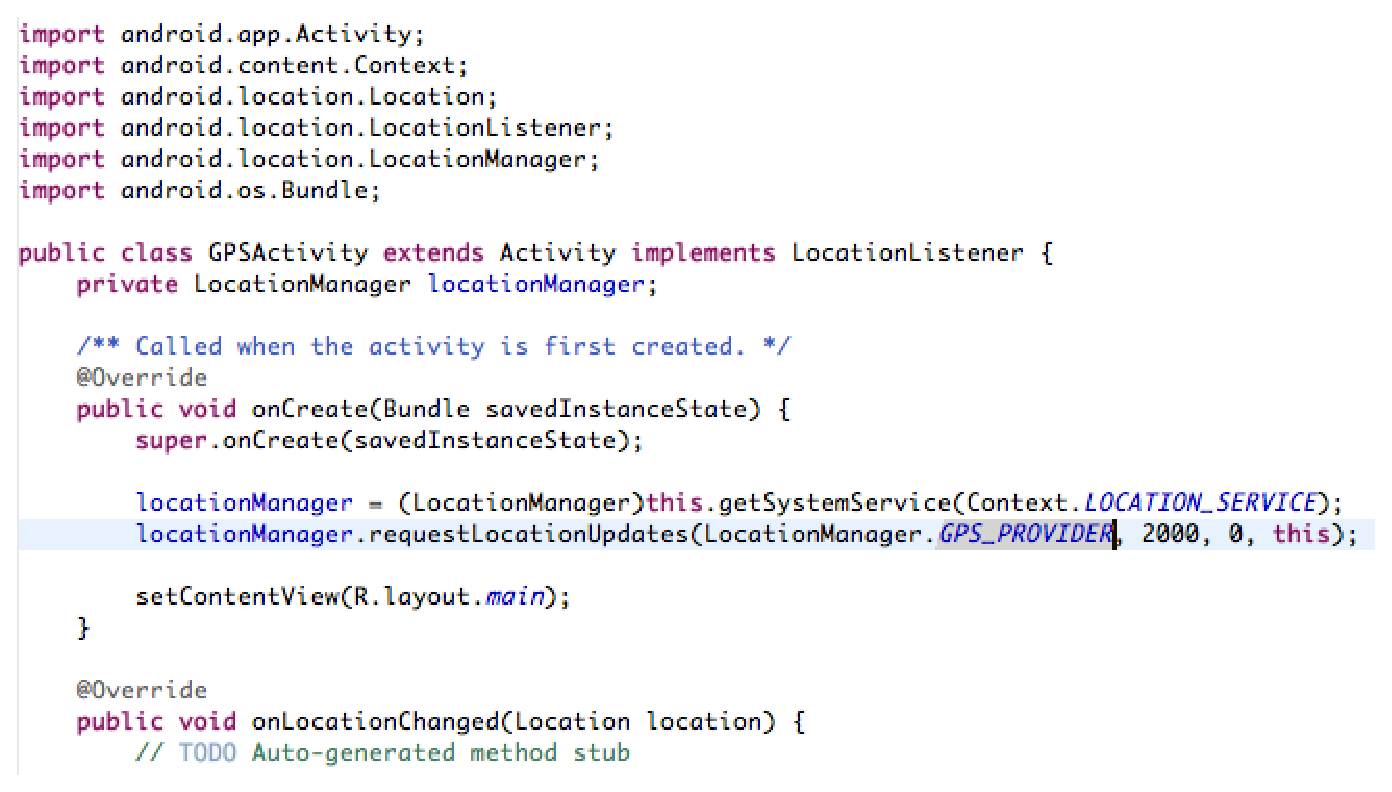
\includegraphics[scale=0.25]{locationListener.eps}
\end{center}

\section*{実装例}
\bigskip
\begin{itemize}
\item 位置情報を Log 出力してみる
\bigskip
\item 地図との連携
\bigskip
\item 住所に変換して出力してみましょう (自力
\end{itemize}

\section*{Log 出力}
\begin{itemize}
\item 出力してみましょう
\end{itemize}
\begin{center}
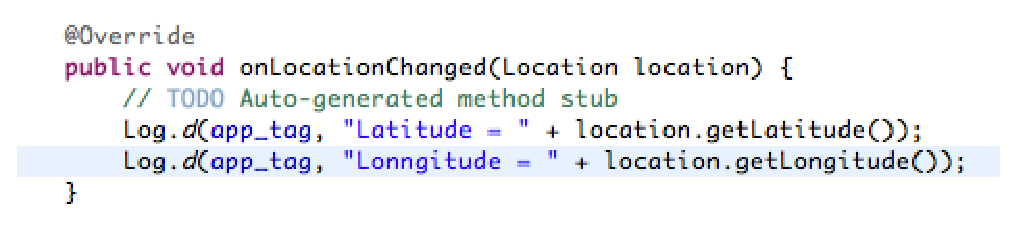
\includegraphics[scale=0.4]{locationLog.eps}
\end{center}

\section*{動かす前に}
\bigskip
\begin{itemize}
\item {\scriptsize GPS デバイスのリスンは明示的に止める必要あり}
 \begin{itemize}
 \item {\scriptsize onPause() で停止 (removeUpdates)}
 \medskip
 \item {\scriptsize onResume() で開始 (requestLocationUpdates)}
 \end{itemize}
\medskip
\item {\scriptsize 画面も固定した方が良い (onCreate、onStop 呼び出しを防ぐ)}
\medskip
\item {\scriptsize ログ出力までに若干時間がかかります}
\end{itemize}

\section*{サンプル}
\bigskip
\begin{itemize}
\item 取得可能な情報を全部出力してみます
 \begin{itemize}
 \item 緯度、軽度
 \item 標高
 \item 速度
 \end{itemize}
\bigskip
\item http://db.tt/zSSCCV
\end{itemize}

\section*{地図との連携 (準備)}
\bigskip
\begin{itemize}
\item MapView と MapController オブジェクトの取得
 \begin{itemize}
 \item MapView オブジェクトの生成
 \item setClickable する
 \item setBuiltInZoomControls する
 \item \begin{verbatim}MapView#getController でオブジェクト取得\end{verbatim}
 \end{itemize}
\end{itemize}

\section*{地図との連携 (onLocationChanged)}
\bigskip
\begin{itemize}
\item GeoPoint オブジェクト生成
 \begin{itemize}
 \item 緯度と軽度を取得して 1E6 を掛けて int にキャスト
 \end{itemize}
\bigskip
\item \begin{verbatim}MapController#animateTo に渡す\end{verbatim}
\end{itemize}

\section*{カメラの取り扱い}
Under Construction

\section*{センサ}
Under Construction

\end{document}
